\section{Review on Graph Theory  }
\textcolor{red}{The definitions stated on this section is based on the book \textit{Graph Theory: Modeling, Applications, and Algorithms} by G. Agnarsson and R. Greenlaw. Reference is on \cite{agnarsson2006graph}.}

\subsection{Preliminaries}
\begin{itemize}
\item \textbf{set} - a group of objects\\
\textcolor{red}{Ex. $A=\{1,2,3,4,5,6,7\}$,$B=\{2,4,6,8,10,12\}$ }
\item \textbf{element} - an object inside a set
\item \textbf{empty set} - null set;contains no element; denoted by $\varnothing$ or $\{\}$
\item If n element $a$ is in set $S$, then $a \in S $.
\item If a set $t$ contains some or all the elements of a set S, then $t \subseteq S$.\\
Ex. If $A=\{1,2,3,4\}$ and $t=\{2,3\}$, then $t \subseteq S$.
\item If set $S$ contains all the elements of $T$ and vice-versa, then $t=S$.\\
Ex. If $A=\{1,2,3,4\}$ and $t=\{1,2,3,4\}$ then $t=S$
\item Let $A$ and $B$ be sets,
\begin{itemize}
	\item $A \cup B$ or the \textit{union of A and B} is the set that contains elements or objects that belong to either $A$ or to $B$ or to both.
	\begin{figure}[h]
	\centering
	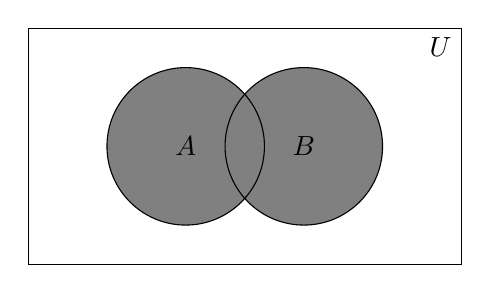
\begin{tikzpicture}
\draw (-2,-1.5) rectangle (3.5,1.5) node[below left]{$U$};
\fill[gray] (0,0) circle (1cm);
\fill[gray] (1.5,0) circle (1cm);
\draw (0,0) circle (1cm) node {$A$};
\draw (1.5,0) circle (1cm) node {$B$};
\end{tikzpicture}
\caption{\textcolor{red}{$A \cup B$ on a Venn Diagram}}
	\end{figure}
	\item $A \cap B$ or the \textit{intersection of A and B} is the set containing the element/s that are present in both $A$ and $B$.
	\begin{figure}[h]
	\centering
	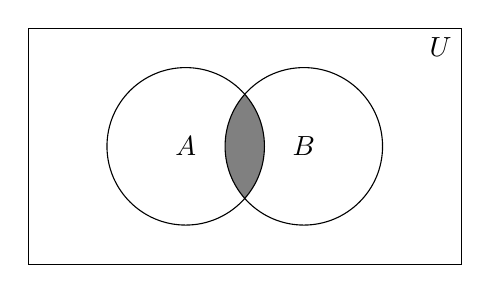
\begin{tikzpicture}
\draw (-2,-1.5) rectangle (3.5,1.5) node[below left]{$U$};
\begin{scope}
\clip (0,0) circle (1cm);
\fill[gray] (1.5,0) circle (1cm);
\end{scope}
\draw (0,0) circle (1cm) node {$A$};
\draw (1.5,0) circle (1cm) node {$B$};
\end{tikzpicture}
\caption{\textcolor{red}{$A \cap B$ on a Venn Diagram}}
	\end{figure}
	\item $A$ an $B$ are disjoint sets if they have no same elements. Disjoint sets can be written as $A \cap B=\varnothing$.
	\begin{figure}[h]
	\centering
	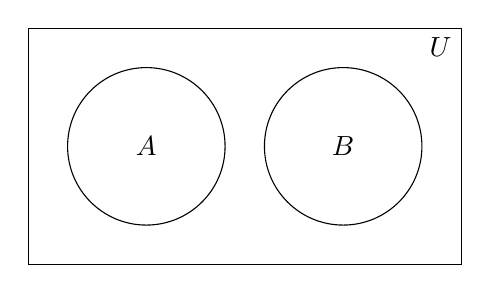
\begin{tikzpicture}
\draw (-2,-1.5) rectangle (3.5,1.5) node[below left]{$U$};
\draw (-0.5,0) circle (1cm) node {$A$};
\draw (2,0) circle (1cm) node {$B$};
\end{tikzpicture}
\caption{\textcolor{red}{Disjoint sets $A$ and $B$ on a Venn Diagram}}
	\end{figure}
	\item $A \setminus B$ or the \textit{set difference of A and B} is the set containing all the elements of $A$ that are not in $B$.
	\textcolor{red}{
	\begin{itemize}
		\item If $A=B$, then $A \setminus B=\varnothing$.
		\item If $A=\varnothing$, then in any $B$, $A \setminus B=\varnothing$.
	\end{itemize}
	}
	\begin{figure}[h]
	\centering
	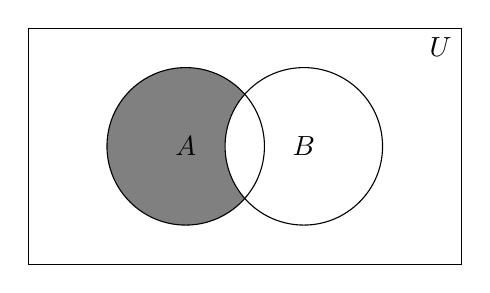
\begin{tikzpicture}
\draw (-2,-1.5) rectangle (3.5,1.5) node[below left]{$U$};
\fill[gray] (0,0) circle (1cm);
\begin{scope}
\clip (0,0) circle (1cm);
\fill[white] (1.5,0) circle (1cm);
\end{scope}
\draw (0,0) circle (1cm) node {$A$};
\draw (1.5,0) circle (1cm) node {$B$};
\end{tikzpicture}
\caption{\textcolor{red}{$A \setminus B$ on a Venn Diagram}}
	\end{figure}
	\item $A \Delta B$ or the \textit{symmetric difference of A and B} is  the set containing the elements of set $A$ that are not in set $B$ combined (union) with the set containing the elements of set $B$ that are not in set $A$. It can be written as $(A \setminus B) \cup (B \setminus A)$. 
\end{itemize}
\begin{figure}[h]
	\centering
	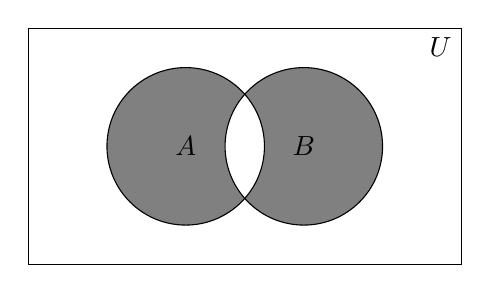
\begin{tikzpicture}
\draw (-2,-1.5) rectangle (3.5,1.5) node[below left]{$U$};
\fill[gray] (0,0) circle (1cm);
\fill[gray] (1.5,0) circle (1cm);
\begin{scope}
\clip (0,0) circle (1cm);
\fill[white] (1.5,0) circle (1cm);
\end{scope}
\draw (0,0) circle (1cm) node {$A$};
\draw (1.5,0) circle (1cm) node {$B$};
\end{tikzpicture}
\caption{\textcolor{red}{$A \Delta B$ on a Venn Diagram}}
	\end{figure}

 \item \textbf{finite set} - a countable set; set that contains countable number elements
 \item  \textbf{cardinality of set $S$ or $|S|$} - the number of elements of set $S$\\
 \textcolor{red}{Ex. Let $A=\{1,3,5,7,9,11,13,15\}$, then $|A|=8$}
 \item \textbf{power set of $S$ or $P(S)$} - the set that all the possible subsets of S including the empty set\\
 \textcolor{red}{Ex. Let $B=\{0,1\}$, then $P(B)=\{\varnothing,0,1,01\}$ and $|P(B)|=4$}
 \item Let $k \in \mathbb{N}$ and $a_1,a_2,...,a_k$ are any k number of objects; \textit{ordered k-tuple or k-tuple} can be written as $(a_1,a_2,...,a_k)$.
 \item Some sets of numbers:
 \begin{itemize}
 	\item set of natural numbers or $\mathbb{N} = \{1,2,3,...\}$
 	\item integer set or $\mathbb{Z} = \{...,-2,-1,0,1,2,...\}$
 	\item set of rational numbers or $\mathbb{Q} = \{a/b:a,b \in \mathbb{Z},b\neq 0 \}$
 	\item set of real numbers or $\mathbb{R}$
 \end{itemize}
\end{itemize}

\subsection{Graphs}
\begin{itemize}
 \item \textbf{graph or general graph} - ordered triple $G=(V,E,\phi)$ where, $V\neq\varnothing$, $V \cap E = \varnothing$ and $\phi:E \rightarrow P(V)$ such that \textcolor{red}{$|\phi(e)|={1,2}$} for every $e \in E$.
 \item Let G be a graph with $G = (V,E,\phi)$,
	\begin{itemize}
		\item The vertex set or $V$ is the set of vertices of G
		\item The edge set or $E$ is the set of edges
		\item $\phi(e)$ contains the endvertex/endvertices of each $e$ which are the elements of the vertex set. 
	\end{itemize}	 
\begin{figure}[h]
\centering
\begin{tikzpicture}[-,>=stealth',shorten >=1pt,auto,node distance=3cm,
                    thick,main node/.style={circle,draw,font=\sffamily\Large\bfseries}]

  \node[main node] (1) {$v_1$};
  \node[main node] (2) [below left of=1] {$v_2$};
  \node[main node] (3) [below of=1] {$v_3$};
  \node[main node] (4) [below right of=1] {$v_4$};
  \node[main node] (5) [below of=3] {$v_5$};
  \node[main node] (6) [right of=4] {$v_6$};
  
  \path[every node/.style={font=\sffamily\large}]
    (1) edge node [right] {$e_3$} (4)
    	edge node [left] {$e_1$} (2)
    	edge node {$e_2$} (3)
    (2) edge [loop left] node {$e_6$} (2)
    (3) edge [bend right] node  {$e_4$} (5)
        edge node [right] {$e_7$} (4)
        edge [bend left,pos=0.2] node  {$e_8$} (5)
    (4) edge node {$e_5$} (5)
	(5) 
    ;
\end{tikzpicture}
\caption{\textcolor{red}{Graph G with 6 vertices and 7 edges.}}
\label{graph1}
\end{figure}
In figure \ref{graph1}, 
\begin{equation}
\begin{array}{l}
G=(V,E,\phi) \\
V=\{v_1,v_2,v_3,v_4,v_5,v_6\} \\
E=\{e_1,e_2,e_3,e_4,e_5,e_6,e_7\} \\
\phi(e_1)=\{v_1,v_2\} \\
\phi(e_2)=\{v_1,v_3\} \\
\phi(e_3)=\{v_1,v_4\} \\
\phi(e_4)=\{v_3,v_5\} \\
\phi(e_5)=\{v_4,v_5\} \\
\phi(e_6)=\{v_2\} \\
\phi(e_7)=\{v_3,v_4\}
\end{array}
\end{equation}
\newpage
Let the graph $G=(V,E,\phi)$,
	\begin{itemize}
\item The vertices $u$ and $v$ are in $V$ and are \textit{adjacent/neighbor} of each other , if there is some edge $e \in E$ that has $\phi(e)=\{u,v\}$ or $\{v,u\}$. In figure 1, $v_1$ and $v_2$ are neighbors.
\item The edges $e_1$ and $e_2$ are in $E$ and are \textit{adjacent} if they contain atleast one same endvertex on their respective $\phi$, such that $\phi\{e_1\} \cap \phi\{e_2\} \neq 0$. In figure 1, $e_1$ and $e_2$ are adjacent
\item Vertex $v$ and edge $e$ are in $V$ and $E$ respectively and are \textit{incident}, if $v$ is in $\phi(e)$. In figure 1, $v_1$ and $e_3$ are incident.
\textcolor{red}{
\item \textbf{Loop} is an edge $e$ with the same endvertices given that $|\phi(e)|=1$. In the figure, $e_2$ is a loop because $\phi(e)=\{v_2\}$
\item $E'$ is a edge set with \textit{multiple/parallel edges}, if $|E'| \leq 2$ and for any edges $e$ and $f$ in $E'$, $\phi(e)=\phi(f)$. In figure, $E'=\{e_4,e_8\}$ because $\phi(e_4)=\phi(e_8)=\{v_3,v_5\}$
}
\item The vertex $v$ is \textit{isolated} if $v$ is not in $\phi(e)$ for all $e$ in $E$
	\end{itemize}
	\item A \textbf{simple graph} is a graph without multiple/parallel edges or loops.
	\item A graph $G=(V,E)$ is a simple graph if,
	\begin{enumerate}
		\item $V\neq\varnothing$
		\item $E=\varnothing$
		\item $E=\{\{v_1,v_2\}:v_1,v_2 \in V, v_1 \neq v_2\}$
	\end{enumerate}
	\begin{figure}[h]
	\centering
\begin{tikzpicture}[-,>=stealth',shorten >=1pt,auto,node distance=3cm,
                    thick,main node/.style={circle,draw,font=\sffamily\Large\bfseries}]

  \node[main node] (1) {$v_1$};
  \node[main node] (2) [below left of=1] {$v_2$};
  \node[main node] (3) [below right of=1] {$v_3$};
  \node[main node] (4) [above right of=1] {$v_4$};
  
  \path[every node/.style={font=\sffamily\large}]
    (1) edge node [right] {$e_1$} (2)
    	edge node [left] {$e_2$} (3)
    	edge node {$e_4$} (4)
    (2) 
    (3) edge node {$e_3$} (4)
        
    (4) 
    ;
\end{tikzpicture}
		\caption{An example of simple graph}
	\end{figure}
	Some examples of Common graphs:
	\item A graph $G=(V,E)$ is a \textit{null graph} on $n$ vertices if,
		\begin{enumerate}
			\item $V=\{v_1,v_2,...,v_n\}$
			\item $E=\varnothing$
		\end{enumerate}
		\begin{figure}[h]
			\centering
			\begin{tikzpicture}[-,>=stealth',shorten >=1pt,auto,node distance=2cm,
                    thick,main node/.style={circle,draw,font=\sffamily\Large\bfseries}]

  \node[main node] (1) {$v_1$};
  \node[main node] (2) [right of=1] {$v_2$};
  \node[main node] (3) [right of=2] {$v_3$};
  \node[main node] (4) [right of=3] {$v_4$};
  
    ;
\end{tikzpicture}
\caption{An example of a null graph on 4 vertices}
		\end{figure}
		
	\item A graph $G=(V,E)$ is a \textit{path graph} on $n\geq2$ vertices if,
		\begin{enumerate}
			\item $V=\{v_1,v_2,...,v_n\}$
			\item $E=\{\{u_1,u_2\},\{u_2,u_3\},...,\{u_{n-1},u_{n}\}\}$
		\end{enumerate}
		
		\begin{figure}[h]
		\centering
		\begin{tikzpicture}[-,>=stealth',shorten >=1pt,auto,node distance=3cm,
                    thick,main node/.style={circle,draw,font=\sffamily\Large\bfseries}]

  \node[main node] (1) {$v_1$};
  \node[main node] (2) [right of=1] {$v_2$};
  \node[main node] (3) [right of=2] {$v_3$};
  \node[main node] (4) [right of=3] {$v_4$};
  
  \path[every node/.style={font=\sffamily\large}]
    (1) edge node {$e_1$} (2)
    (2) edge node {$e_2$} (3)
    (3) edge node {$e_3$} (4)  
    (4) 
    ;
\end{tikzpicture}
\caption{An example of a path graph one 4 vertices}
		\end{figure}
	\item A graph $G=(V,E)$ is a \textit{cycle graph or cycle} on $n\geq3$ vertices if,
	\begin{enumerate}
		\item $V=\{v_1,v_2,...,v_n\}$
		\item $E=\{\{v_1,v_2\},\{v_2,v_3\},...,\{v_{n-1},v_{n}\},\{v_n,v_1\}\}$
	\end{enumerate}
	\begin{figure}[h]
	\centering
	\begin{tikzpicture}[-,>=stealth',shorten >=1pt,auto,node distance=3cm,
                    thick,main node/.style={circle,draw,font=\sffamily\Large\bfseries}]

  \node[main node] (1) {$v_1$};
  \node[main node] (2) [right of=1] {$v_2$};
  \node[main node] (3) [below right of=2] {$v_3$};
  \node[main node] (4) [below left of=3] {$v_4$};
  \node[main node] (5) [left of=4] {$v_5$};
  \node[main node] (6) [above left of=5] {$v_6$};
  
  \path[every node/.style={font=\sffamily\large}]
    (1) edge node {$e_1$} (2)
    (2) edge node {$e_2$} (3)
    (3) edge node {$e_3$} (4)  
    (4) edge node {$e_4$} (5)
    (5) edge node {$e_5$} (6)
    (6) edge node {$e_6$} (1)
    ;
\end{tikzpicture}
	
	\caption{An example of a cycle graph on 6 vertices}
	\end{figure}
	\item A graph $G=(V,E)$ is a \textit{complete graph} on $n$ vertices if,
	\begin{enumerate}
		\item $V=\{v_1,v_2,...,v_n\}$
		\item $E=\{\{v_i,v_j\}:1\leq i \leq j \leq n\}$
	\end{enumerate}
	\begin{figure}[h]
	\centering
	\begin{tikzpicture}[-,>=stealth',shorten >=1pt,auto,node distance=3cm,
                    thick,main node/.style={circle,draw,font=\sffamily\Large\bfseries}]

  \node[main node] (1) {$v_1$};
  \node[main node] (2) [right of=1] {$v_2$};
  \node[main node] (3) [below right of=2] {$v_3$};
  \node[main node] (4) [below left of=3] {$v_4$};
  \node[main node] (5) [left of=4] {$v_5$};
  \node[main node] (6) [above left of=5] {$v_6$};
  
  \path[every node/.style={font=\sffamily\large}]
    (1) edge node {} (2)
    	edge node {} (3)
    	edge node {} (4)
    	edge node {} (5)
    	edge node {} (6)
    (2) edge node {} (3)
    	edge node {} (4)
    	edge node {} (5)
    	edge node {} (6)
    (3) edge node {} (4)
    	edge node {} (5)
    	edge node {} (6)  
    (4) edge node {} (5)
    	edge node {} (6)
    (5) edge node {} (6)
    (6)
    ;
\end{tikzpicture}
	
	\caption{An example of a complete graph on 6 vertices}
	\end{figure}
	\item A graph is a \textit{complete bipartite (m,n)-graph} on $m+n$ vertices, if
	\begin{enumerate}
		\item $V=\{s_1,s_2,...,s_m\} \cup \{v_1,v_2,...,v_n\}$
		\item $E=\{\{s_i,v_j\}:1\leq i \leq m, 1 \leq j \leq n\}$
	\end{enumerate}	
	\begin{figure}[h]
	\centering
	\begin{tikzpicture}[-,>=stealth',shorten >=1pt,auto,node distance=3cm,
                    thick,main node/.style={circle,draw,font=\sffamily\Large\bfseries}]

  \node[main node] (1) {$v_1$};
  \node[main node] (2) [right of=1] {$v_2$};
  \node[main node] (3) [right of=2] {$v_3$};
  \node[main node] (4) [right of=3] {$v_4$};
  \node[main node] (5) [below left of=1] {$s_1$};
  \node[main node] (6) [below right of=1] {$s_2$};
  \node[main node] (7) [below right of=2] {$s_3$};
  \node[main node] (8) [below right of=3] {$s_4$};
  \node[main node] (9) [below right of=4] {$s_5$};
  
  \path[every node/.style={font=\sffamily\large}]
    (1) edge node {} (5)
    	edge node {} (6)
    	edge node {} (7)
    	edge node {} (8)
    	edge node {} (9)
    (2) edge node {} (5)
    	edge node {} (6)
    	edge node {} (7)
    	edge node {} (8)
    	edge node {} (9)
    (3) edge node {} (5)
    	edge node {} (6)
    	edge node {} (7)
    	edge node {} (8)
    	edge node {} (9)  
    (4) edge node {} (5)
    	edge node {} (6)
    	edge node {} (7)
    	edge node {} (8)
    	edge node {} (9)
    ;
\end{tikzpicture}
\caption{An example of a complete bipartite $(4,5)$-graph on $4+5$ vertices}
\end{figure}	 
\end{itemize}
\subsection{Degrees and Regular Graph}
Let $G=(V,E,\phi)$ be a graph with vertex $v\in V$,
\begin{itemize}

	\item $d_G(v)$ or $d(v)$ (when there is no other given graphs) is the \textit{degree of the vertex $v$} given by,
	$$d(v)=|\{e\in E: v \in \phi(e), |\phi(e)|=1,2 \}|$$
	It is the cardinality of edges that are connected to the vertex $v$.\\ 
	Some Remarks:\\  \\
	\begin{tabular}{|l|l|} \hrulefill
		Type of Graph & $d(v)$ \\  \hrulefill
		Simple & number of neighbors of $v$ \\  \hrulefill
		Loopless & number of edges that have $v$ as endvertex \\  \hrulefill
		General & same as loopless but loops are counted twice \\  \hrulefill
	\end{tabular}
	\item The set $N_G(v)$ or $N(v)$ is called the \textit{open neighborhood of v} or the \textit{neighborhood of v}.It is the set of all the vertex neighbors of the vertex $v$ in graph $G$. It is given by,
		$$N(v)=\{w \in V: \phi(e)=\{v,w\} or \{w,v\}, e \in E\}$$
	\item Additionally, the \textit{closed neighborhood of v}  denoted by $N[v]$  is the set of all the elements in the open neighbor with the vertex $v$ itself. 
	$$N[v]=N(v) \cup v$$
	
\begin{figure}[h]
	\centering
	\begin{tikzpicture}[-,>=stealth',shorten >=1pt,auto,node distance=3cm,
                    thick,main node/.style={circle,draw,font=\sffamily\Large\bfseries}]

  \node[main node] (1) {$v_1$};
  \node[main node] (2) [below left of=1] {$v_2$};
  \node[main node] (3) [below right of=1] {$v_3$};
  \node[main node] (4) [right of=3] {$v_4$};
  
  \path[every node/.style={font=\sffamily\large}]
    (1) edge node {} (2)
    	edge node {} (3)
    (2) edge [bend left]node {} (3)
    	edge [loop left] node {} (2)
    (3) edge [bend left] node {} (2)
    	edge node {} (4)
    (4) 
    ;
\end{tikzpicture}
\caption{An example of a graph with various degrees.}
\label{degreefig}
\end{figure}

In figure \ref{degreefig}, 
\begin{equation}
\begin{array}{c c}
d(v_1)=2 & N(v_1)=\{v_2,v_3\} \\
d(v_2)=5 & N(v_2)=\{v_1,v_3\}\\
d(v_3)=4 & N(v_3)=\{v_1,v_2,v_4\}\\
d(v_4)=1 & N(v_4)=\{v_3\}\\
N[v_1]=N[v_2]=\{v_1,v_2,v_3\} & N[v_3]=V\\
N[v_4]=\{v_3,v_4\}

\end{array}
\end{equation}
\\ \\
 \item Hand Shake Theorem \\ The \textit{hand shake theorem} was inspired from the hand shaking scenario on a party. Each person in the party needs to shake hands with the other persons in the room. The amount of shake hands made is twice the number of persons in the party. In parallel to graphs, people in the party represents the vertex set of the graph and the shake hands made are the edge set of the graph. The graph $G=(V,E)$ has a total degree of,
 $$\sum\limits_{u\in V} d(v) = 2|E|$$
	\item The graph $F=(V',E',\phi')$ is a subset of graph $G=(V,E,\phi)$ if,
	\begin{enumerate}
		\item $V' \subseteq V$,
		\item $E' \subseteq E$,
		\item $\phi'(e) = \phi(e) \forall e \in E'$	
	\end{enumerate}	 
	The subgraph relationship is denoted by $\subseteq$. So that, we can say $F \subseteq G$
\begin{figure}[h]
	\centering
	\begin{tikzpicture}[-,>=stealth',shorten >=1pt,auto,node distance=3cm,
                    thick,main node/.style={circle,draw,font=\sffamily\Large\bfseries}]

  \node[main node] (1) {$v_1$};
  \node[main node] (2) [below right of=1] {$v_2$};
  \node[main node] (3) [below left of=1] {$v_3$};
  \node[main node] (4) [above left of=3] {$v_4$};
  \node[main node] (5) [left of=3] {$v_5$};
  
  \path[every node/.style={font=\sffamily\large}]
    (1) edge node {} (2)
    	edge node {} (4)
    	edge node {} (5)
    (2) 
    (3) edge node {} (4)
    	edge node {} (5)
    (4) edge node {} (5)
    (5)
    ;
\end{tikzpicture}

\begin{tikzpicture}[-,>=stealth',shorten >=1pt,auto,node distance=3cm,
                    thick,main node/.style={circle,draw,font=\sffamily\Large\bfseries}]

  \node[main node] (1) {$v_1$};
  \node[main node] (3) [below left of=1] {$v_3$};
  \node[main node] (4) [above left of=3] {$v_4$};
  \node[main node] (5) [left of=3] {$v_5$};
  
  \path[every node/.style={font=\sffamily\large}]
    (1)	edge node {} (4)
    	edge node {} (5)
    (2) 
    (3) edge node {} (4)
    	edge node {} (5)
    (4) edge node {} (5)
    (5)
    ;
\end{tikzpicture}
\caption{The graph $F$ (bottom) is a subgraph of graph $G$ (top). }
\label{subgraphfig}
\end{figure}	
\end{itemize}	
\subsection{Directed Graphs}
\begin{itemize}
	\item A \textit{directed graph or digraph} is an ordered triple given by $G=(V,E,\eta)$ where,
	\begin{enumerate}
		\item $V \neq \varnothing$
		\item $V \cap E = \varnothing$
		\item $\eta:E \mapsto V \times V$
	\end{enumerate}
	\begin{itemize}
		\item $V$ is the vertex set
		\item $E$ is the set of directed edges
		\item If $u,v \in V$,$e \in E$ and $\eta(e)=(u,v)$, then $u$ is the tail of $e$ and $v$ is the head of $e$.
	\end{itemize}
	\begin{figure}[h]
	\centering
	\begin{tikzpicture}[->,>=stealth',shorten >=1pt,auto,node distance=3cm,
                    thick,main node/.style={circle,draw,font=\sffamily\Large\bfseries}]

  \node[main node] (1) {$v_1$};
  \node[main node] (2) [right of=1] {$v_2$};
  \node[main node] (3) [below left of=2] {$v_3$};
  \node[main node] (4) [below of=2] {$v_4$};
  \node[main node] (5) [below of=3] {$v_5$};
  
  \path[every node/.style={font=\sffamily\large}]
    (1) edge node {$e_1$} (2)
    	
    (2) edge node {$e_2$} (4)
    (3) edge node {$e_3$} (2)
    (4) edge node {$e_4$} (5)
    (5) edge node {$e_5$} (3)
    ;
\end{tikzpicture}
\caption{An example of a directed graph.}
\label{digraphfig}
\end{figure}
In figure \ref{digraphfig}, 
\begin{equation}
\begin{array}{c}
V=\{v_1,v_2,v_3,v_4,v_5\}, \\
E=\{e_1,e_2,e_3,e_4,e_5\}, \\
\eta(e_1)=(v_1,v_2), \\
\eta(e_2)=(v_2,v_4), \\
\eta(e_3)=(v_3,v_2), \\
\eta(e_4)=(v_4,v_5), \\
\eta(e_5)=(v_5,v_3), \\
\end{array}
\end{equation}
\textcolor{red}{
\item A graph is a \textit{path digraph} on $n\leq2$ vertices, where
\begin{enumerate}
	\item $V=\{u_1,u_2,...,u_n\}$
	\item $E=\{e_1,e_2,...,e_{n-1}\}$
	\item $\eta(e_1)=(u_i,u_{i+1})$ for all $i \in \{1,...,n-1\}$
\end{enumerate}
}
\begin{figure}[h]
	\centering
	\begin{tikzpicture}[->,>=stealth',shorten >=1pt,auto,node distance=3cm,
                    thick,main node/.style={circle,draw,font=\sffamily\Large\bfseries}]

  \node[main node] (1) {$v_1$};
  \node[main node] (2) [above right of=1] {$v_2$};
  \node[main node] (3) [below right of=2] {$v_3$};
  \node[main node] (4) [above right of=3] {$v_4$};
  
  \path[every node/.style={font=\sffamily\large}]
    (1) edge node {$e_1$} (2)
    (2) edge node {$e_2$} (3)
    (3) edge node {$e_3$} (4)
    ;
\end{tikzpicture}
\caption{\textcolor{red}{An example of a \textit{path digraph on 4 vertices}.}}
\label{pathdigraphfig}
\end{figure}
\textcolor{red}{
\item A graph is a \textit{cycle digraph} on $n\leq1$ vertices, where
\begin{enumerate}
	\item $V=\{u_1,u_2,...,u_n\}$
	\item $E=\{e_1,e_2,...,e_{n-1},e_n\}$
	\item $\eta(e_1)=(u_i,u_{i+1})$ for all $i \in \{1,...,n-1\}$
	\item $\eta(n)=(u_n,u_1)$
\end{enumerate}
}
\begin{figure}[h]
	\centering
	\begin{tikzpicture}[->,>=stealth',shorten >=1pt,auto,node distance=3cm,
                    thick,main node/.style={circle,draw,font=\sffamily\Large\bfseries}]

  \node[main node] (1) {$v_1$};
  \node[main node] (2) [above right of=1] {$v_2$};
  \node[main node] (3) [below right of=2] {$v_3$};
  
  \path[every node/.style={font=\sffamily\large}]
    (1) edge node {$e_1$} (2)
    (2) edge node {$e_2$} (3)
    (3) edge node {$e_3$} (1)
    ;
\end{tikzpicture}
\caption{\textcolor{red}{An example of a \textit{cycle digraph on 3 vertices}.}}
\label{pathdigraphfig}
\end{figure}
\textcolor{red}{
\item A graph is a \textit{simple digraph} if it has no directed loops and no parallel edges. Figure \ref{digraphfig} is an example of a simple digraph since it has no directed loops and no parallel edges.}
\end{itemize}


\subsection{\textcolor{red}{Degrees of Digraph}}

Let $G=(V,E,\eta)$ be a digraph and vertex $u \in V$ ,
\begin{itemize}
	\item The \textit{indegree of u} denoted by $d_G^-(u)$ or $d^-(u)$ is the number of directed edges having $u$ as a head, that is,\\
	\begin{center}
	$d^-(u)=|\{e \in E: \eta(e)=(x,u)$ for some $ x \in V\}|$
	\end{center}
	
	\item The \textit{outdegree of u} denoted by $d_G^+(u)$ or $d^+(u)$ is the number of directed edges having $u$ as a head, that is,\\
	\begin{center}
	$d^+(u)=|\{e \in E: \eta(e)=(u,y)$ for some $ y \in V\}|$
	\end{center}
	\item The \textit{inneighbors of u} denoted by $N_G^-$ or $N^-$ is given by,
	\begin{center}
	$N^-(u)=\{x \in V: \eta(e)=(x,u)$ for some $ e \in E\}$
	\end{center}
	\item The \textit{outneighbors of u} denoted by $N_G^+$ or $N^+$ is given by,
	\begin{center}
	$N^+(u)=\{x \in V: \eta(e)=(u,y)$ for some $ e \in E\}$
	\end{center}
	\item 
	\begin{center}
		$\sum\limits_{u\in V} d^-(u) = \sum\limits_{u\in V} d^+(u)=|E|$
	\end{center}
\end{itemize}

\subsection{Paths, Cycles and Weights}
Let $G=(V,E,\phi)$ be a graph with $V=\{v_1,v_2,...,v_k\}$ and $E=\{e_1,e_2,...,e_k\}$ as its vertex and edge set respectively, then,
\begin{enumerate}
	\item A \textbf{walk} in graph G is the alternating sequence of edges and vertices that start and stops with a vertex given by,
	$(v_1,e_1,v_2,e_2,...,e_k,v_k)$ such that $\phi(e_j)=\{v_{j-1},v_j\}$ for $j \in k$.
	\item A trail in G is a walk with all of its edges to be distinct.
	\item A path in G is a walk with all of its vertices to be distinct.
	\item A $u-v$ walk/trail/path is a walk starting from  the vertex $u$ and ends on the vertex $v$ with their respective characteristics.
	\item A $v-v$ walk/trail is a circuit (or closed walk/trail).
	\item A $v-v$ path is a cycle.\\
	\begin{figure}[h]
	\centering
	\begin{tikzpicture}[-,>=stealth',shorten >=1pt,auto,node distance=3cm,
                    thick,main node/.style={circle,draw,font=\sffamily\Large\bfseries}]

  \node[main node] (1) {$v_1$};
  \node[main node] (2) [right of=1] {$v_2$};
  \node[main node] (3) [below left of=1] {$v_3$};
  \node[main node] (4) [right of=2] {$v_4$};
  \node[main node] (5) [below right of=3] {$v_5$};
  \node[main node] (6) [right of=5] {$v_6$};
  
  \path[every node/.style={font=\sffamily\large}]
    (1) edge node {$e_1$} (2)
    	edge [bend left] node {$e_2$} (3)
    	edge node {$e_3$} (5)
    	edge node {$e_4$} (6)
    (2) edge node {$e_5$} (4)
    (3) edge node {$e_6$} (5)
    	edge [bend left] node{$e_7$} (1)
    (4) edge node {$e_8$} (6)
    (5) edge node {$e_9$} (6)
    (6)
    ;
\end{tikzpicture}
\caption{An example of a graph to show walks,trails,paths and cycles.}

\label{walkfig}
\end{figure}
\item[] In figure \ref{walkfig},
\begin{itemize}
\item $q=(v_1,e_2,v_3,e_7,v_1,e_4,v_6,e_4,v_1,e_1,v_2,e_5,v_4)$\\ $q$ is a walk of length 6. $q$ is not a trail since $e_4$ is repeated. $q$ is not also a path because $v_1$ appeared many times.
\item $r=(v_3,e_2,v_1,e_7,v_3,e_6,v_5,e_9,v_6,e_8,v_4)$ \\ $r$ is a walk of length 5 and a trail because there are no repeating edges. $r$ is no a path because the vertex $v_3$ is repeated.
\item $t=(v_1,e_1,v_2,e_5,v_4,e_8,v_6,e_9,v_5)$ \\ $t$ is a path of length 4 because there are no repeating vertices in the walk.
\item $d=(v_1,e_1,v_2,e_5,v_4,e_8,v_6,e_9,v_5,e_3,v_1)$ \\ $d$ is a closed walk, closed trail and a cycle of length 5.
\end{itemize}
\item \textcolor{red}{Let $G$ be a graph and $W: E \rightarrow \mathbb{R}$, the ordered tuple $(G,W)$ is called a \textit{weighted graph}. The function $W$ is called a \textit{weight/weight function} of $(G,W)$.}
\begin{figure}[h!]
	\centering
\begin{tikzpicture}[->,>=stealth',shorten >=1pt,auto,node distance=3cm,
                    thick,main node/.style={circle,draw,font=\sffamily\Large\bfseries}]

  \node[main node] (1) {$v_1$};
  \node[main node] (2) [below left of=1] {$v_2$};
  \node[main node] (3) [below right of=1] {$v_3$};
  \node[main node] (4) [above right of=1] {$v_4$};
  
  \path[every node/.style={font=\sffamily\large}]
    (1) edge node [right] {$1.2$} (2)
    	edge node [left] {$0.6$} (3)
    	edge node {$1.33$} (4)
    (2) 
    (3) edge node {$0.4$} (4)
        
    (4) 
    ;
\end{tikzpicture}
		\caption{An example of a weighted simple digraph}
		\label{wgraph}
	\end{figure}
\\ \\In figure \ref{wgraph},
	\begin{equation}
		\begin{array}{c}
			W((v_1,v_2))=1.2\\
			W((v_1,v_3))=0.6\\
			W((v_1,v_4))=1.33\\
			W((v_3,v_4))=0.4
		\end{array}
	\end{equation}
\end{enumerate}

%\subsection{Connectivity, Isomorphism and Homomorphism}
%\begin{itemize}
%	\item A graph $G=(V,E,\phi)$ is \textit{connected} if, for every unique pair vertices $u,v \in V$, $G$ has a $u,v$-path. Otherwise, $G$ is \textit{disconnected}.
%	\item Let $G=(V,E,\phi)$ and $G'=(V',E',\phi')$ be graphs. A \textit{homomorphism} $f:G \rightarrow G'$ from $G$ to $G'$ is an ordered pair $f=(f_1,f_2)$ of maps, $f_1:V \rightarrow V'$ and $f_2=E \rightarrow E'$, also satisfying the compatibility condition, $$\phi(e)=\{u,v\} \implies \phi'(f_2(e))= \{f_1(u),f_1(v)\} $$
%	So if $u$ and $v$ are envertices of an edge $e$ in $G$, then $f_1(u)$ and $f_21(v)$ must also be the end vertices of edge $f_2(e)$ in $G'$.
%\end{itemize}



\section{Introduction to the Problem}"Viral Marketing" is a term first introduced in 1997 by Steve Jurvetson and Time Draper\cite{viralmarketing}. It is an effective way of advertising a product to a large group of people by having little groups eventually spread awareness to your product. Companies make a commercial with this in mind. Many over-the-top and absurd commercial having been making rounds across the internet \cite{commercialrise}. First, being seen by a few people who were entertained by the commercial enough for them to hit the share button creating a network to other people who will eventually see the commercial shared by their friend and promptly clicking the share button themselves. Thus, repeating the cycle and expanding the network. 

Online social networks are a good medium to advertise on. Viral Marketing on online social networks is a very cost-effective technique that most companies today utilize. For only spending a few dollars, the payoff can be amazing.\cite{viralmarketing} In 1996, this strategy was used by the once popular e-mail service Hotmail: Every mail sent via Hotmail contained advertisement for the service. A total of \$50,000 was spent on this campaign. Hotmail expanded into 12 million users in just 18 months.\cite{viralmarketing} 

Recently, the video game company Epic Games, used this tactic to advertise their new battle royale game "Fortnite" and it gave astounding results. The number one video streaming site, Youtube, is a very large network and resource to put to use. They sponsored Youtubers with hundred to millions of subscribers to promote their game.\cite{sponsoredvideos} Youtuber Evan Fong "VanossGaming" was one of the content creators Epic Games sponsored for advertising the beta release of Fortnite \cite{vanoss}. He currently has 23 million subscribers(August 2018). The video, titled "Fortnite Funny Moments-Launcing the Rocket!(Gameplay)", has garnered 10 million views in a span of a year.

With this in mind, finding the set of people to target would be ideal. \textbf{Target Set Selection} is basically finding the smallest set of people in a social network to influence all of the people in said network.\cite{Kempe,chen,Shakarian:2012:LSN:2456719.2457081} This network can be represented with a graph $G$ with each person as a node/vertex $V$. Connecting each node/vertex $V$ is an edge $E$. Connected vertices are considered neighbors $n$. The degree $d(v)$ of each node is how many neighbors a node has. The threshold $k(v)$ of each node is a factor to gauge the suceptability of a node from being influenced. The neighbor $N(v)$ is the set of neighbors of the node. 

\subsection{Two Basic Diffusion Models}
\textcolor{red}{A diffusion model is a set mathematical formulas that attempt to model the spread of information or a disease through a network or population}

Two basic diffusion models have been introduced in 2003 by Kempe, Kleinberd and Tardos.\cite{Kempe} These models are improved upon by works proceeding it. These two models are considered in order to further understand the basics and foundations of the models the algorithm is based/taken from.


In the following models, as information spreads through the network nodes will be referred to as either $active$ or $inactive$. The chance of the node to be active increases as more of its neighbor become active. Inactive nodes can become active nodes but the other way around is not to be considered. 

\textcolor{red}{
Imagine yourself walking down the street. A stranger approaches you and hands you a brochure showing you how amazing a new product is, but still, it's not enough to convince you to buy said product. As you walk home, you see a poster with your favorite celebrity advertising the same product. You think: \textit{"That seems nice, I'll consider buying it"}. You arrive to see your parents using the same product. So you quickly leave your house to buy the product. The next day, you tell your friends about the product you just bought and try to make them buy and use it.}

\textcolor{red}{
We represent the different vertices in the network graph as the stranger, the poster of the celebrity or your parents, each having individual weights on your decision to buy the product. You start off as unconvinced(inactive) that the product is worth buying, but as time goes by and as the influence of other people pile up on you, you reach your threshold and finally buy the product, making you active. Making you eligible to influence other inactive nodes/vertices.}

\textcolor{red}{
We also assume that a node can only switch from inactive to active and not the other way around. A active node will remain active during the diffusion process. The process runs until no more activation occurs.\cite{Shakarian:2012:LSN:2456719.2457081} }
\subsubsection{Linear Threshold Model}
\textcolor{red}{Different people have different weights to their words. If a family member or a famous person gives you a recommendation, we assume that their statement will have a large weight attributed to it and if a random stranger you do not know and have no affiliation with tell you to buy their product, we know that it will have tiny to average effect on you the consumer.}

Given a simple directed graph $G=(V,E)$, we assign a weight $w\in \mathbb{R}^{+}$ on each edge $e$ selected uniformly random in the interval $[0,1]$. We also assign a threshold $t \in \mathbb{R}^{+}$ to every vertex in $G$ selected uniformly random in the interval $[0,1]$.
We define a vertex/node as active when

		$$\sum_{e \in \eta^{in}(v)} w(e)\geq t(v)$$

If the sum of the weight of the edges incoming to the vertex $v$ is greater than or equal to the threshold of $v$, $v$ becomes active. \textcolor{red}{The process ends when all nodes are active.}

\textcolor{red}{
In the first graph in the figure \ref{linearfig} we set to vertex C to be active to start the process. After each time step/round $r$ we look to see if the weight of the edges outgoing from the activated vertices to the other vertices in its neighborhood. At round 2 vertices B and D become active. At round 3 A becomes active and the process ends when all the vertices are active. 
\cite{Kempe} 
}
\begin{figure}[h!]
	\begin{minipage}{0.45\textwidth}
		\begin{tikzpicture}[->,>=stealth',shorten >=1pt,auto,node distance=4cm,
                    thick,main node/.style={circle,draw,font=\sffamily\small\bfseries}]

  \node[main node,label={0.4}] (A) {$A$};
  \node[main node,label={0.8},color={red}] (C) [below of=A] {$C$};
  \node[main node,label={0.6}] (B) [right of=A] {$B$};
  \node[main node,label={0.3}] (D) [right of=C] {$D$};
  
  \path[every node/.style={font=\sffamily\large}]
    (A) edge node {$0.5$} (B)
    	edge node {$0.4$} (C)
    (B) edge node {$0.2$} (A)
    	edge node {$0.3$} (C)
    	edge node {$0.2$} (D)
    (C) edge node {$0.3$} (A)
    	edge node {$0.7$} (B)
    	edge node {$0.5$} (D)
    (D) edge node {$0.3$} (C)
    	edge node {$0.4$} (B)
    ;
		\end{tikzpicture}
		\caption{r=1}
	\end{minipage}
	\begin{minipage}{0.45\textwidth}
		\begin{tikzpicture}[->,>=stealth',shorten >=1pt,auto,node distance=4cm,
                    thick,main node/.style={circle,draw,font=\sffamily\small\bfseries}]

  \node[main node,label={0.4}] (A) {$A$};
  \node[main node,label={0.8},color={red}] (C) [below of=A] {$C$};
  \node[main node,label={0.6},color={red}] (B) [right of=A] {$B$};
  \node[main node,label={0.3},color={red}] (D) [right of=C] {$D$};
  
  \path[every node/.style={font=\sffamily\large}]
    (A) edge node {$0.5$} (B)
    	edge node {$0.4$} (C)
    (B) edge node {$0.2$} (A)
    	edge node {$0.3$} (C)
    	edge node {$0.2$} (D)
    (C) edge node {$0.3$} (A)
    	edge node {$0.7$} (B)
    	edge node {$0.5$} (D)
    (D) edge node {$0.3$} (C)
    	edge node {$0.4$} (B)
    ;
\end{tikzpicture}
\caption{r=2}

	\end{minipage}
	\vspace*{0.2cm}
	\begin{minipage}{0.45\textwidth}
	\centering
		\begin{tikzpicture}[->,>=stealth',shorten >=1pt,auto,node distance=4cm,
                    thick,main node/.style={circle,draw,font=\sffamily\small\bfseries}]

  \node[main node,label={0.4}, color={red}] (A) {$A$};
  \node[main node,label={0.8},color={red}] (C) [below of=A] {$C$};
  \node[main node,label={0.6}, color={red}] (B) [right of=A] {$B$};
  \node[main node,label={0.3}, color={red}] (D) [right of=C] {$D$};
  
  \path[every node/.style={font=\sffamily\large}]
    (A) edge node {$0.5$} (B)
    	edge node {$0.4$} (C)
    (B) edge node {$0.2$} (A)
    	edge node {$0.3$} (C)
    	edge node {$0.2$} (D)
    (C) edge node {$0.3$} (A)
    	edge node {$0.7$} (B)
    	edge node {$0.5$} (D)
    (D) edge node {$0.3$} (C)
    	edge node {$0.4$} (B)
    ;
\end{tikzpicture}
\caption{r=3}
	\end{minipage}
\caption{Linear Threshold model of graph G at $r=1,2,3$ with C initially activated}
\label{linearfig}
\end{figure}

\subsubsection{Independent Cascade Model}
\textcolor{red}{Now, in this model, we assume that when a person tries you influence you, they only have that one chance to do so. After that, they lose their chance of doing it again. We still have the knowledge that different people have different weights assigned to their words. In this model, however, we assign a percentage that determines how likely is that person to influence you. Say, your mother has a 90\% chance to recommend you a product but, on the contrary, the known scam artist has a 15\% chance of influencing you.}

Given a simple directed graph $G(V,E)$,we assign a probability $P_{u,v}$, this defines the probability of $u$ infecting $v$. Each node can try to influence its neighbor. When a node is influenced successfully, the node being influenced becomes active. If a node fails to influence a neighbor they cannot try to influence that node again.\cite{Kempe}\cite{Shakarian:2012:LSN:2456719.2457081}
\begin{figure}[h!]
	\begin{minipage}{0.45\textwidth}
		\begin{tikzpicture}[->,>=stealth',shorten >=1pt,auto,node distance=4cm,
                    thick,main node/.style={circle,draw,font=\sffamily\small\bfseries}]

  \node[main node] (A) {$A$};
  \node[main node,color={red}] (C) [below of=A] {$C$};
  \node[main node] (B) [right of=A] {$B$};
  \node[main node] (D) [right of=C] {$D$};
  
  \path[every node/.style={font=\sffamily\large}]
    (A) edge node {$0.1$} (B)
    	edge node {$0.4$} (C)
    (B) edge node {$0.5$} (A)
    	edge node {$0.6$} (C)
    (C) edge node {$0.3$} (A)
    	edge node {$0.2$} (B)
    	edge node {$0.5$} (D)
    (D) edge node {$0.2$} (C)
    	
    ;
\end{tikzpicture}
\caption{r=1}
	\end{minipage}
	\begin{minipage}{0.45\textwidth}
		\begin{tikzpicture}[->,>=stealth',shorten >=1pt,auto,node distance=4cm,
                    thick,main node/.style={circle,draw,font=\sffamily\small\bfseries}]

  \node[main node,color={gray}] (A) {$A$};
  \node[main node,color={red}] (C) [below of=A] {$C$};
  \node[main node,color={red}] (B) [right of=A] {$B$};
  \node[main node,color={gray}] (D) [right of=C] {$D$};
  
  \path[every node/.style={font=\sffamily\large}]
    (A) edge node {$0.1$} (B)
    	edge node {$0.4$} (C)
    (B) edge node {$0.5$} (A)
    	edge node {$0.6$} (C)
    (C) edge node {$0.3$} (A)
    	edge node {$0.2$} (B)
    	edge node {$0.5$} (D)
    (D) edge node {$0.2$} (C)
    ;
\end{tikzpicture}
\caption{r=2}
	\end{minipage}
	\begin{minipage}{0.45\textwidth}
		\centering
	\begin{tikzpicture}[->,>=stealth',shorten >=1pt,auto,node distance=4cm,
                    thick,main node/.style={circle,draw,font=\sffamily\small\bfseries}]

  \node[main node, color={red}] (A) {$A$};
  \node[main node,color={red}] (C) [below of=A] {$C$};
  \node[main node, color={red}] (B) [right of=A] {$B$};
  \node[main node, color={gray}] (D) [right of=C] {$D$};
  
  \path[every node/.style={font=\sffamily\large}]
    (A) edge node {$0.1$} (B)
    	edge node {$0.4$} (C)
    (B) edge node {$0.5$} (A)
    	edge node {$0.6$} (C)
    (C) edge node {$0.3$} (A)
    	edge node {$0.2$} (B)
    	edge node {$0.5$} (D)
    (D) edge node {$0.2$} (C)
    ;
\end{tikzpicture}
\caption{r=3}
	\end{minipage}
\caption{Independent Cascade model of graph G at $r=1,2,3$ with C initially activated}
\label{Independentfig1}
\end{figure}

\textcolor{red}{
Notice that on figure \ref{Independentfig1}; at round 2, vertex $C$ fails to activate vertices A and D. This means that C loses the ability to influence said vertices but this doesn't mean that that the neighbor of vertex A can't influence A. At round 3, vertex B succeeds in influencing vertex A and all of the vertices have been tried for activation and there they have no more neighbors left to activate, meaning, the process ends.}
\subsection{The threshold model reintroduced by Chen}

Now, we limit and modify the model. Where in the vertices/nodes know each other or have some kind of connection/relationship. This means, every neighbor or friend of a certain person has the same effect as every other neighbor or friend of that person. The threshold is only thing to be considered. When determining how likely a person is to be influence, the size of their neighbor considered.

Given a simple undirected connected graph $G=(V,E)$, let $d(v)$ to be the degree of $v \in V$. For each node/vertex $v \in V$, we assign a threshold value $t(v) \in \mathbb{N}$, where $1 \leq t(v) \leq d(v)$. At the start, the states of all the nodes/vertices are set to inactive. We then pick a subset of $V$, the $target\; set$, and set their states to active. At each round/time step, the states of vertices are to be updated if an inactive vertex $v$ has at least as many active neighbors as its threshold $t(v)$. The process ends when all vertices are active or no additional vertices can make the remaining nodes active. Again, the vertices can only change states from being inactive to active, not the other way around \cite{chen}.

The difference of this model to the two previously discussed models by Kempe et.al \cite{Kempe}\cite{Shakarian:2012:LSN:2456719.2457081}, is that their model focused on maximization of the vertices the target set can activate. This model on the other hand, will aim to find a target set that activates all or a fixed fraction of vertices. The previous two models were based of probabilistic thresholds where all thresholds were drawn randomly from a given distribution. \cite{Kempe}\cite{chen}

\begin{figure}[h!]
	\centering
	\begin{minipage}{0.45\textwidth}
		\begin{tikzpicture}[-,>=stealth',shorten >=1pt,auto,node distance=4cm,
                    thick,main node/.style={circle,draw,font=\sffamily\small\bfseries}]

  \node[main node,label={$3$}] (A) {$A$};
  \node[main node,color={red},label=below:{$3$}] (C) [below of=A] {$C$};
  \node[main node,label={$1$}] (B) [right of=A] {$B$};
  \node[main node,label=below:{$1$}] (D) [right of=C] {$D$};
  
  \path[every node/.style={font=\sffamily\large}]
    (A) edge node {} (B)
    	
    (B) 
    (C) edge[color=red] node {} (A)
    	edge[color=red] node {} (D)
    (D) edge node {} (B)
    	edge node {} (A)
    	
    ;
\end{tikzpicture}
\caption{r=1}
	\end{minipage}
	\centering
	\begin{minipage}{0.45\textwidth}
		\begin{tikzpicture}[-,>=stealth',shorten >=1pt,auto,node distance=4cm,
                    thick,main node/.style={circle,draw,font=\sffamily\small\bfseries}]

  \node[main node,label={$3$}] (A) {$A$};
  \node[main node,color={red},label=below:{$3$}] (C) [below of=A] {$C$};
  \node[main node,label={$1$}] (B) [right of=A] {$B$};
  \node[main node,label=below:{$1$},color={red}] (D) [right of=C] {$D$};
  
  \path[every node/.style={font=\sffamily\large}]
    (A) edge node {} (B)
    	
    (B) 
    (C) edge[color=red] node {} (A)
    	edge[color=red] node {} (D)
    (D) edge[color=red] node {} (B)
    	edge[color=red] node {} (A)
    	
    ;
\end{tikzpicture}
\caption{r=2}
	\end{minipage}
	\centering
	\begin{minipage}{0.45\textwidth}
		\begin{tikzpicture}[-,>=stealth',shorten >=1pt,auto,node distance=4cm,
                    thick,main node/.style={circle,draw,font=\sffamily\small\bfseries}]

  \node[main node,label={$3$}] (A) {$A$};
  \node[main node,color={red},label=below:{$3$}] (C) [below of=A] {$C$};
  \node[main node,label={$1$},color={red}] (B) [right of=A] {$B$};
  \node[main node,label=below:{$1$},color={red}] (D) [right of=C] {$D$};
  
  \path[every node/.style={font=\sffamily\large}]
    (A) edge[color=red] node {} (B)
    	
    (B) 
    (C) edge[color=red] node {} (A)
    	edge[color=red] node {} (D)
    (D) edge[color=red] node {} (B)
    	edge[color=red] node {} (A)
    	
    ;
\end{tikzpicture}
\caption{r=3}
	\end{minipage}
	\centering
	\begin{minipage}{0.45\textwidth}
		\begin{tikzpicture}[-,>=stealth',shorten >=1pt,auto,node distance=4cm,
                    thick,main node/.style={circle,draw,font=\sffamily\small\bfseries}]

  \node[main node,label={$3$},color={red}] (A) {$A$};
  \node[main node,color={red},label=below:{$3$},color={red}] (C) [below of=A] {$C$};
  \node[main node,label={$1$},color={red}] (B) [right of=A] {$B$};
  \node[main node,label=below:{$1$},color={red}] (D) [right of=C] {$D$};
  
  \path[every node/.style={font=\sffamily\large}]
    (A) edge[color=red] node {} (B)
    	
    (B) 
    (C) edge[color=red] node {} (A)
    	edge[color=red] node {} (D)
    (D) edge[color=red] node {} (B)
    	edge[color=red] node {} (A)
    	
    ;
    

\end{tikzpicture}
\caption{r=4}
	\end{minipage}

\caption{Threshold model with C vertex as target set at round/time step = 1,2,3,4}
\label{Thresholdfig1}
\end{figure}

\textcolor{red}{
In the example figure \ref{Thresholdfig1}, we pick C as the target set. We activate C at round 1. At round 2 we check the neighbors of C which is A and D, but only D is eligible for activation since the threshold of A is 3 and it does not have enough active neighbors. D, however is eligible for activation and activates at round 2. In the next round, B, with threshold 1, activates since D is active and is a neighbor of B. Finally at round 4, A has enough active neighbors to reach its threshold 3.}

\textcolor{red}{In the two previous diffusion models, we assign a value to the edges of the directed graph. This means that the neighbors of that vertices have different strengths of influence to a certain node. In Chen's model, the neighbors of any vertex $v \in V$ all have the same strength in influencing said vertex. The threshold will depend on how weak or strong a vertex is from being influenced.}

The threshold value is set depending on the network we want to find the target set of.

\begin{enumerate}
	\item \textbf{Small Thresholds} This case is when all the thresholds are small constants. However, this threshold becomes more complex as the threshold increases from $k=1$. Past researches have studied that, for any $k \leq 2$, the Target Set Selection Problem is NP-hard.A statement constructed by Chen et.al(2009) states that the Target Set Selection problem is NP-hard when the thresholds are at most 2. Earlier before that, Dreyer(2000) proved this instance for only $k \geq 3$.\cite{dreyer} \cite{NPhardness} 
	\begin{itemize}
	\item Time Complexity defines the runtime of a certain algorithm. Denoted by the Big-O notation. Example: $O(n)$ is linear time, $n$ represents the size of the input.
	\item P or Polynomial time is a set of languages that are relatively easy to get the solution and to verify it (i.e Multiplication, sorting, finding primes, etc). This determined from the time complexity of the algorithm. Being in polynomial time, the notation would be $O(n^k)$ for some $k>1$.
	\item NP or Non-deterministic polynomial time is the set of languages that can verified in polynomial time. Basically NP Problems are problems that when given a solution, it is easy to verify the solution, but hard to get the solution itself.
	\item NP-Complete problems are problems that are in NP and are NP-hard(i.e $n^{2}by\; n^{2}$ sudoku, Boolean Satisfiability Problem). They are also considered as the hardest problems in NP.
	\item A problem is NP-hard if the problem is atleast as hard or even harder than the problems in NP. This means that if you find an algorithm that solves an NP-hard problem, you can use that very algorithm to solve any other problem in NP in polynomial time or P = NP(i.e Cryptography, Routing, Scheduling).  
\end{itemize} 
\textbf{The Target Set Selection problem is NP-hard when the threshold $k$ for every vertex $v$ is at most 2}. \cite{chen,dreyer}

For the instance of $k=1$ it can be solved trivially. Take any graph $G$ and set of all node's thresholds $k=1$. Activate any of the nodes in that graph and you will create a chain reaction of activating \textbf{every} node in that graph. So, with $k=1$ we can take any one node from that graph that is our target set.\cite{chen}

This is commonly used in study of social networks where in an action of a small group of people is enough to make their neighbor pick up same behavior/principle/ideology.
	\textcolor{red}{
	\item \textbf{Majority Thresholds t=$\frac{d(v)}{2}$} One important and well-studied threshold model is the majority threshold. This is where a vertex becomes active if at least half of its neighbors are active [1,$\frac{d(v)}{2}$].\cite{chen} This can be applied to networks that have voting systems, dynamic monopolies, distributed computing and use the majority rule. It was proven by Peleg (1997) that this type of threshold value is NP-hard. \cite{majority} }
	
	\textcolor{red}{
	\item \textbf{Unanimous Thresholds t(v)=d(v)} This setting is considered the most influence-resistant of the previously mentioned.\cite{chen} All the nodes have unanimous thresholds meaning, the threshold of each node is the same as it's degree. This threshold can be applied to an ideal virus-resistant network, where a vertex is infected only if all of its neighbors are infected with the virus. With this in mind, this threshold can be used in constructing robust virus resistant network structures.\cite{chen} }
\end{enumerate}

\subsection{Target Set Selection Algorithms compared in this study}

\subsubsection{TIP-DECOMP}
\begin{algorithm}
	\caption{TIP-DECOMP}
	\begin{algorithmic}[1]
		\Require Threshold function, $t$ and social network $G=(V,E)$
		\Ensure $V'$
		
		\ForAll{$vertex \  v_{i}$}
			\State compute $k_{i}$ 
		\EndFor
		\ForAll{$vertex \  v_{i}$}
			\State $dist_{i}=d_{i}^{in}-k_{i} $
		\EndFor
		\State FLAG=TRUE 
		\While{FLAG=TRUE}
			\For{$v_{i} \in V $}
				\If{$v_{i}\; has \;min(dist_{i})$}
					\State $v_{i}=$ current $v$
				\EndIf
			\EndFor
			\If{$dist_{i}=\infty$}
				\State FLAG=FALSE 
			\Else
			\State Remove $v_{i}$ from $G$ 
				\ForAll{$v_{j} \in n_{i}^{out}$} 
					\If {$dist_{j}>0$}  
						\State $dist_{j}=dist_{j}-1$
					\Else
						\State$dist_{j}=\infty$  
					\EndIf
				\EndFor
			\EndIf
		\EndWhile
		\State \Return All nodes left in G 
	\end{algorithmic}
\end{algorithm}

\begin{itemize}
	\item $d_{i}^{in}$= degree of vertex $v_{i}$
	\item At lines 1-3, a for loop is used for computing the $k_{i}'s$ for each vertex $v_{i}$. $k_{i}$ is defined as  $k_{i}=[t(v_{i})\cdot d_{i}^{in}]$
	\item At lines 4-6, a for loop is used to compute for the distribution or $dist_{i}$. This will later be used as distinguishing what the current $v_{i}$ is to be used in the inner while loop.
	\item At line 7 a FLAG is instantiated as a boolean variable which will be used in the while loop for identifying the target set selection. We can see it being used in line 8.
	\item The for loop in line 9-13 is for selecting the vertex $v_{i}$ where the result of the degree and the threshold is minimal.
	\item Lines 14-16 are for escaping the main while loop. If this condition is met, it means that the procedure is done.
	\item The else statement in 16-25 is for removing the vertex where the degree and the threshold is almost the same(line 17).
	\item The inner for loop in lines 18-24 is used for updating the distributions in the neighborhood of $v_{j}$.
	\item The process returns the reduced vertex set with the vertices removed if necessary. This is the target set.
\end{itemize}
TIP-DECOMP or Tipping Decomposition is model based on the idea of node "tipping" when a node adopts a property or behavior if a number of his neighbors currently exhibit the same. It is a type of Target Set Selection Algorithm. 

The algorithm above inputs a threshold function $t$ and the social network $G$ and outputs the network with vertices removed based off the condition in the algorithm.\cite{tipdecomp}

\subsubsection{Step by step example}
\begin{figure}[h!]
\centering
	\begin{tikzpicture}[-,>=stealth',shorten >=1pt,auto,node distance=2cm,
                    thick,main node/.style={circle,draw,font=\sffamily\small\bfseries}]

  \node[main node,label={right:$v_1$}] (1) {$2$};
  \node[main node,label={above right:$v_2$}, below of=1] (2) {$4$};
  \node[main node,label={right:$v_3$}, below left of=2] (3) {$1$};
  \node[main node,label={below:$v_4$}, below of=2] (4) {$1$};
  \node[main node,label={right:$v_5$}, below right of=2] (5) {$2$};
  \node[main node,label={right:$v_6$},right of=2] (6) {$1$};
  \node[main node,label={right:$v_7$},above right of=6] (7) {$2$};
  \node[main node,label={right:$v_8$},above left of=7] (8) {$1$};
  \node[main node,label={right:$v_9$},below of=7] (9) {$3$};
  \node[main node,label={right:$v_{10}$},below of=9] (10) {$1$};
  
  
  \path[every node/.style={font=\sffamily\large}]
    (1) edge node {} (2)
    (2) edge node {} (3)
    	edge node {} (4)
    	edge node {} (5)
    	edge node {} (6)
    (3) 
    (4) edge node {} (10)
    (5) edge node {} (9)
    (6) edge node {} (7)
    (7) edge node {} (8)
    	edge node {} (9)
    (8)	edge node {} (1)
    (9) edge node {} (10)
    (10) 
    
    ;
\end{tikzpicture}
\end{figure}
\begin{table}[ht]
\centering
    \begin{tabular}{c c c c c}
		Vertex $v_{i}$ & Degree $d^{in}_{i}$ & Threshold $t_{i}$& $k_{i}$ & $dist_{i}$\\
		$v_{1}$ & 2 & 2 & 4 & -2 \\
		$v_{2}$ & 5 & 4 & 20 & -15\\
		$v_{3}$ & 1 & 1 & 1 & 0\\
		$v_{4}$ & 2 & 1 & 2 & 0\\
		$v_{5}$ & 2 & 2 & 4 & -2\\
		$v_{6}$ & 2 & 1 & 2 & 0\\
		$v_{7}$ & 3 & 2 & 6 & -3\\
		$v_{8}$ & 2 & 1 & 2 & 0\\
		$v_{9}$ & 3 & 3 & 9 & -6\\
		$v_{10}$ & 2 & 1 & 2 & 0\\
	\end{tabular}
\end{table}
   
 \begin{figure}
 
 We first choose the vertex with minimum $dist$ which in this case is $v_{2}$, we remove $v_{2}$ from the graph and update the $dist$ of their neighbors. We set the $dist$ of the vertices with 0 or negative $dist$ values as $\infty$, meaning they are the maximum or not considered in the selection of current $v$.
 \begin{minipage}{0.45\textwidth}
 	
	\begin{tikzpicture}[-,>=stealth',shorten >=1pt,auto,node distance=2cm,
                    thick,main node/.style={circle,draw,font=\sffamily\small\bfseries}]

  \node[main node,label={right:$v_1$}] (1) {$2$};
  \node[main node,label={right:$v_3$}, below left of=2] (3) {$1$};
  \node[main node,label={below:$v_4$}, below of=2] (4) {$1$};
  \node[main node,label={right:$v_5$}, below right of=2] (5) {$2$};
  \node[main node,label={right:$v_6$},right of=2] (6) {$1$};
  \node[main node,label={right:$v_7$},above right of=6] (7) {$2$};
  \node[main node,label={right:$v_8$},above left of=7] (8) {$1$};
  \node[main node,label={right:$v_9$},below of=7] (9) {$3$};
  \node[main node,label={right:$v_{10}$},below of=9] (10) {$1$};
  
  
  \path[every node/.style={font=\sffamily\large}]
    (1)
    (3) 
    (4) edge node {} (10)
    (5) edge node {} (9)
    (6) edge node {} (7)
    (7) edge node {} (8)
    	edge node {} (9)
    (8)	edge node {} (1)
    (9) edge node {} (10)
    (10) 
    
    ;
\end{tikzpicture}
\end{minipage}
\begin{minipage}{0.45\textwidth}
    \begin{tabular}{c c c c c}
		Vertex $v_{i}$ & Degree $d^{in}_{i}$ & Threshold $t_{i}$& $k_{i}$ & $dist_{i}$\\
		$v_{1}$ & 2 & 2 & 4 & $\infty$ \\
		$v_{3}$ & 1 & 1 & 1 & $\infty$\\
		$v_{4}$ & 2 & 1 & 2 & $\infty$\\
		$v_{5}$ & 2 & 2 & 4 & $\infty$\\
		$v_{6}$ & 2 & 1 & 2 & $\infty$\\
		$v_{7}$ & 3 & 2 & 6 & -3\\
		$v_{8}$ & 2 & 1 & 2 & 0\\
		$v_{9}$ & 3 & 3 & 9 & -6\\
		$v_{10}$ & 2 & 1 & 2 & 0\\
	\end{tabular}

\end{minipage}
\noindent\makebox[\linewidth]{\rule{\paperwidth}{0.4pt}}
\vspace*{0.5cm}  
\begin{minipage}{0.45\textwidth}
 	
	\begin{tikzpicture}[-,>=stealth',shorten >=1pt,auto,node distance=2cm,
                    thick,main node/.style={circle,draw,font=\sffamily\small\bfseries}]

  \node[main node,label={right:$v_1$}] (1) {$2$};
  \node[main node,label={right:$v_3$}, below left of=2] (3) {$1$};
  \node[main node,label={below:$v_4$}, below of=2] (4) {$1$};
  \node[main node,label={right:$v_5$}, below right of=2] (5) {$2$};
  \node[main node,label={right:$v_6$},right of=2] (6) {$1$};
  \node[main node,label={right:$v_7$},above right of=6] (7) {$2$};
  \node[main node,label={right:$v_8$},above left of=7] (8) {$1$};
  \node[main node,label={right:$v_{10}$},below of=9] (10) {$1$};
  
  
  \path[every node/.style={font=\sffamily\large}]
    (1)
    (3) 
    (4) edge node {} (10)
    (5) 
    (6) edge node {} (7)
    (7) edge node {} (8)
    (8)	edge node {} (1)
    (10) 
    
    ;
\end{tikzpicture}
\end{minipage}
\begin{minipage}{0.45\textwidth}
    \begin{tabular}{c c c c c}
		Vertex $v_{i}$ & Degree $d^{in}_{i}$ & Threshold $t_{i}$& $k_{i}$ & $dist_{i}$\\
		$v_{1}$ & 2 & 2 & 4 & $\infty$ \\
		$v_{3}$ & 1 & 1 & 1 & $\infty$\\
		$v_{4}$ & 2 & 1 & 2 & $\infty$\\
		$v_{5}$ & 2 & 2 & 4 & $\infty$\\
		$v_{6}$ & 2 & 1 & 2 & $\infty$\\
		$v_{7}$ & 3 & 2 & 6 & $\infty$\\
		$v_{8}$ & 2 & 1 & 2 & 0\\
		$v_{10}$ & 2 & 1 & 2 & $\infty$\\
	\end{tabular}

\end{minipage}
\noindent\makebox[\linewidth]{\rule{\paperwidth}{0.4pt}}
\vspace*{0.5cm} 

Only $\infty \; dist$ values are left thus, stopping the process. The nodes left in the graph the target set according to the algorithm.
\begin{minipage}{0.45\textwidth}
 	
	\begin{tikzpicture}[-,>=stealth',shorten >=1pt,auto,node distance=2cm,
                    thick,main node/.style={circle,draw,font=\sffamily\small\bfseries}]

  \node[main node,label={right:$v_1$}] (1) {$2$};
  \node[main node,label={right:$v_3$}, below left of=2] (3) {$1$};
  \node[main node,label={below:$v_4$}, below of=2] (4) {$1$};
  \node[main node,label={right:$v_5$}, below right of=2] (5) {$2$};
  \node[main node,label={right:$v_6$},right of=2] (6) {$1$};
  \node[main node,label={right:$v_7$},above right of=6] (7) {$2$};
  \node[main node,label={right:$v_{10}$},below of=9] (10) {$1$};
  
  
  \path[every node/.style={font=\sffamily\large}]
    (1)
    (3) 
    (4) edge node {} (10)
    (5) 
    (6) edge node {} (7)
    (7)
    (10) 
    
    ;
\end{tikzpicture}
\end{minipage}
\begin{minipage}{0.45\textwidth}
    \begin{tabular}{c c c c c}
		Vertex $v_{i}$ & Degree $d^{in}_{i}$ & Threshold $t_{i}$& $k_{i}$ & $dist_{i}$\\
		$v_{1}$ & 2 & 2 & 4 & $\infty$ \\
		$v_{3}$ & 1 & 1 & 1 & $\infty$\\
		$v_{4}$ & 2 & 1 & 2 & $\infty$\\
		$v_{5}$ & 2 & 2 & 4 & $\infty$\\
		$v_{6}$ & 2 & 1 & 2 & $\infty$\\
		$v_{7}$ & 3 & 2 & 6 & $\infty$\\
		$v_{10}$ & 2 & 1 & 2 & $\infty$\\
	\end{tabular}

\end{minipage}
\end{figure}

\subsection{VirAds} 


\begin{algorithm}
	\caption{VirAds Algorithm}
	\begin{algorithmic}[1]
		
		
		\Require Graph $G = (V,E),0<\rho<1,d\in N^{+}$
		\Ensure A small $d-seeding$ 
		\State $n_{v}^{(e)} = d(v),n_{v}^{(a)} = \rho \cdot d(v), r_{v}  = d + 1, v \in V $
		
		\State $r_{v}^{i}=0, i=0..d, P  = \varnothing $
		
		
		\While{there exist inactive vertices}
		\Repeat
		\State $u  = argmax_{v\not\in P}\{n_{v}^{(e)}+n_{v}^{(a)}\}$ 
		
		Recompute $n_{v}^{(e)}$ as the number of new active edges after adding $u$.
		\Until{$u = argmax_{v\not\in P}\{n_{v}^{(e)}+n_{v}^{(a)}\}$ }
		\State $P  = P \cup \{u\} $
		\State Initialize a queue: $Q  = \{(u,r_{v})\} $
		\State $r_u = 0 $
		\ForAll{$x \in N(u)$}
		
		\State $n_{x}^{(a)}  = max\{n_{x}^{(a)}-1,0\} $
		
		\EndFor
		\While{$Q\not=\varnothing$}
		\State$(t,\widetilde{r_{t}})  = Q.pop() $
		\ForAll{$w \in N(t)$}
		\ForAll{$i=r_{t}\  to$ min $\{\widetilde{r_{t}}-1,r_{w}-2\}$}
		\State $r_{w}^{(i)}=r_{w}^{(i)}+1 $
		\If{$(r_{w}^{(i)}\geq \rho \cdot d_{w})\wedge(r_{w}\geq d)\wedge(i+1<d)$}
		\ForAll{$x\in N(w)$}
		\State $n_{x}^{(a)} =$max$\{n_{x}^{(a)}-1,0\} $	
		\EndFor
		\State $r_{w}=i+1 $
		\If{$w\not\in Q$}
		\State $Q.push(w,r_{w}) $	
		\EndIf
		\EndIf
		\EndFor
		\EndFor
		\EndWhile
		\EndWhile
	\end{algorithmic}
\end{algorithm}
\begin{itemize}
	\item $\rho =$ The influence factor is a decimal between 0-1 that is multiplied to the degree of current vertex $v$ to get $n_{v}^{(a)}$
	\item $r_{v}$ = the round in which the vertex $v$ is activated
	\item $n_{v}^{(e)}=$ the number of new active edges after adding $v$ into the seeding
	\item $n_{v}^{(a)}=$ the number of extra active neighbors $v$ needs in order for it to activate.
	\item $r_{v}^{i}=$ the number of activated neighbors of $v$ up to round $i$ where $i$=$1..d$
	\item Lines 1-2 are for initialization. Line 1 is initialization of variables with values while line 2 is initialization of zero variables.
	\item Line 3 shows that all inactive vertices will be activated or considered in the algorithm
	\item Line 4-6 finds the value where the maximum occurs in the sum of the degree of v and it's effectiveness.
	\item $u$ is added to P in line 7
	\item A queue is initialized by adding the vertex and its corresponding round, which at the start is zero $(u,r_{v})$
	\item Lines 10-12 updates the neighbors of $u$, reducing their degree by 1. If less than zero is reached, it goes back to zero.
	\item At the start of the while loop in line 14 $(t,r_{t})$ is set as the head of the queue. This is obtained by the pop function. 
	\item For all neighbors $w$ of the current node $t$, another for loop is used for checking if the neighbors of $t$ have reached the threshold defined by $\rho \cdot d_{w}$ AND $round \; r_{w} \geq the\; max\; round\; d$ AND the index $i$ of the for loop doesn't exceed the max rounds $d$.
	\item This then leads to the thresholds of the neighbors of the that neighbor $w$ being decremented.
	\item In line 22 the round of the neighbor $w$ is incremented and if that current $w \notin Q$ then it is added to the queue and the while loop starts again.
\end{itemize}
VirAds selects in each step the vertex $u$ with the highest effectiveness which is defined as $n^{(e)}_{u}+n^{(e)}_{(a)}$. Which is basically the vertex $v$ which can activate the most number of $edges$. It also considers the vertex with the most active neighbors. After that, the algorithm updates the measures for all the remaining vertices. VirAds will make the selection based on the information within $d$-hop neighbor around the considered vertices rather than only one-hop neighbor as in the degree-based heuristic. When a vertex $u$ is selected, it causes a chain-reaction and activate a sequence of vertices or lower the rounds in which vertices are activated.\cite{virads}

The algorithm utilizes a queue. A queue is a data structure which is FIFO. Imagine, a line at any commercial establishment where the first who came is the first who's served. 
\section{Main algortihm developed in the study}
\subsection{Preliminaries}
	Let $G = (V,E)$ be a graph modeling a network. $\Gamma$ is the neighborhood of current vertex $v$ and $d_{g}(v)$ or $|\Gamma_{g}(v)|$ as the degree of current vertex $v$.
	Let $t: V \rightarrow N_{0}={0,1,...}$ be the threshold function assigned to the vertices of $G$. For each node $v \in V$, the threshold $t(v)$ indicates how hard or how easy it is to influence vertex $v$. Low thresholds means easier to influence and high thresholds are hard to influence.
	
	The activation process in $G$ starting at $S$ is a sequence of vertex subsets $Active_{G}[S,0] \subseteq Active_{G}[S,1] \subseteq ... \subseteq Active_{G}[S,\ell] \subseteq ... \subseteq V$ of vertex subsets, with $Active_{G}[S,0]=S$ and 
	
	$Active_{G}[S,\ell]=Active_{G}[S,\ell-1] \cup \{u:|\Gamma_{G}(u)\cap Active_{G}[S,\l-1]|\geq t(u)\}, for \; \ell \geq 1$
	
	A target set for $G$ is set $S \subseteq V$ such that $Active_{G}[S,\lambda]=V$ for some $\lambda \geq 0$
	
	This means at each round $\ell$ the set of active nodes is augmented by the set of nodes $u$ that have a number of already activated neighbors greater or equal to $u$'s threshold $t(u)$. The vertex $v$ is said to be activated at round $\ell \ge 0$ if $v \in Active_{G}[S,\ell]\setminus Active_{G}[S,\ell-1]$.
	
	\subsection{The TSS Algorithm}
	
	Given the input graph $G$, at each round/iteration if the vertex has already been considered it will be removed from the graph. When the current vertex $v$ is deleted in the graph its neighbors degree is updated and the current $v$ is removed from the neighbor set of the neighbors of $v$.
	
	If the vertex $v$ is deemed applicable to be in the target set, the thresholds of their neighbors are decreased by one since the deleted node is able to activate them.
	
	In this algorithm 3 cases are considered:
	\begin{itemize}
		\item Case 1: The threshold $k$ of the current vertex $v$ is 0.\\
		The vertex $v$ is activated by the influence of its neighbors in $V - U$ only; it can then influence its neighbors in U.\\
		So, for each neighbor of vertex $v$ denoted by $u$, reduce the threshold of $u$ by 1.
		\item Case 2: The degree of $v$ is less than the its threshold.\\
		The vertex v is added to S, since no sufficient neighbors remain in $U$ to activate it; v can then influence its neighbors in $U$.\\
		Add the current $v$ to S
		For each neighbor of vertex $v$ denoted by $u$, reduce the threshold of $u$ by 1.
		\item Case 3: The other conditions are not met.\\
		The vertex $v$ will be influence by some of its neighbors in $U$.\\
		Set the vertex $v$ as the vertex in which this equation $\frac{k(u)}{\delta(u)(\delta(u)+1)}$.\\ Note: the maximum value that this equation bears when $k(u)=\delta(u)=1$. When 1 is substituted to the equation $\frac{1}{2}$ is obtained. With the threshold and degree of a vertex = 1, the node is a leaf. This implies that for every change of v, the ones with low degrees and threshold are considered first.
		
	\end{itemize}
	
	\subsubsection{Pseudocode of TSS Algorithm}
		\paragraph{Definition of Variables} 
		\begin{itemize}
			\item $S$: target Set
			\item $d(v)$: degree of vertex $v$
 			\item $t(v)$: threshold of vertex $v$
 			\item $Gamma(v)$: neighbor set of vertex $v$
		\end{itemize}
		\begin{algorithm}
			\caption{TSS Algorithm}
			\begin{algorithmic}[1]
				\Require $G=(V,E),$ Thresholds $ t(v)$ for $v\in V$
				\Ensure Target Set $S$
				\State $S=\varnothing$
				\State 
				$U=V$
				\ForAll{$v \in v$}
					\State $\delta(v)=d(v)$
					\State $k(v)=t(v)$
					\State	$N(v)=\Gamma(v)$
				\EndFor
				\While{$U \not = \varnothing$}
					\If{there exists $v\in U \; s.t \; k(v)=0$}
					
					\ForAll{$u \in N{v}$}
						\State$k(u)=max(k(u)-1,0)$
						\State $S=S\cup \{v\}$
					\EndFor
					\Else 
						\If{ there exists $v \in U\; s.t\; \delta(v) \le k(v)$}
						\ForAll{$u \in N(v)$}
						\State $k(u)=k(u)-1$
						\EndFor
						\Else 
							\State $v=argmax_{u\in U}\{\frac{k(u)}{\delta(u)(\delta(u)+1)}\}$
						\EndIf
					\EndIf
					\ForAll{$u \in N(v)$}
						\State $\delta(u)=\delta(u)-1$
						\State $N(u)=N(u)-{v}$
					\EndFor
					\State $U=U-{v}$
				\EndWhile
			\end{algorithmic}
		\end{algorithm}
\newpage
\begin{figure}[h]
	\centering
	\begin{tikzpicture}[-,>=stealth',shorten >=1pt,auto,node distance=3cm,
                    thick,main node/.style={circle,draw,font=\sffamily\small\bfseries}]

  \node[main node,label={right:$v_1$}] (1) {$3$};
  \node[main node,label={right:$v_2$},below of=1] (2) {$1$};
  \node[main node,label={right:$v_3$}, below right of=1] (3) {$1$};
  \node[main node,label={right:$v_4$},above right of=1] (4) {$1$};
  \node[main node,label={right:$v_5$}, below right of=4] (5) {$2$};
  \node[main node,label={right:$v_6$},below of=5] (6) {$1$};
  \node[main node,label={right:$v_7$},below left of=1] (7) {$2$};
  \node[main node,label={right:$v_8$},below left of=7] (8) {$1$};
  \node[main node,label={right:$v_9$},below right of=7] (9) {$1$};
  \node[main node,label={right:$v_{10}$},below of=6] (10) {$1$};
  
  
  
  \path[every node/.style={font=\sffamily\large}]
    (1) edge node {} (7)
    	edge node {} (2)
    	edge node {} (3)
    (2) 
    (3) 
    (4) edge node {} (1)
    	edge node {} (5)
    (5) edge node {} (6)
    (6) edge node {} (10)
    (7) edge node {} (8)
    	edge node {} (9)
    (8)
    (9)
    (10) 
    
    ;
\end{tikzpicture}
\caption{A tree with 10 vertices where the number inside the circle is the vertex threshold.}
\label{degreefig}
\end{figure}
\begin{equation}
\begin{array}{l c c c c c c c c c c}
	Iteration & 1 & 2 & 3 & 4 & 5 & 6 & 7 & 8 & 9 & 10 \\
	vertex & v_{10} & v_9 & v_8 & v_7 & v_6 & v_5 & v_4 & v_3 & v_2 & v_1 \\
	Case & 3 & 3 & 3 & 2 & 3 & 2 & 1 & 3 & 3 & 2\\
\end{array}
\end{equation}
\subsubsection{Step by step example}
\begin{figure}[!h]
	\begin{minipage}{0.45\textwidth}

	\begin{tikzpicture}[-,>=stealth',shorten >=1pt,auto,node distance=2cm,
                    thick,main node/.style={circle,draw,font=\sffamily\small\bfseries}]

  \node[main node,label={right:$v_1$}] (1) {$2$};
  \node[main node,label={above right:$v_2$}, below of=1] (2) {$4$};
  \node[main node,label={right:$v_3$}, below left of=2] (3) {$1$};
  \node[main node,label={below:$v_4$}, below of=2] (4) {$1$};
  \node[main node,label={right:$v_5$}, below right of=2] (5) {$2$};
  \node[main node,label={right:$v_6$},right of=2] (6) {$1$};
  \node[main node,label={right:$v_7$},above right of=6] (7) {$2$};
  \node[main node,label={right:$v_8$},above left of=7] (8) {$1$};
  \node[main node,label={right:$v_9$},below of=7] (9) {$3$};
  \node[main node,label={right:$v_{10}$},below of=9] (10) {$1$};
  
  
  \path[every node/.style={font=\sffamily\large}]
    (1) edge node {} (2)
    (2) edge node {} (3)
    	edge node {} (4)
    	edge node {} (5)
    	edge node {} (6)
    (3) 
    (4) edge node {} (10)
    (5) edge node {} (9)
    (6) edge node {} (7)
    (7) edge node {} (8)
    	edge node {} (9)
    (8)	edge node {} (1)
    (9) edge node {} (10)
    (10) 
    
    ;
\end{tikzpicture}
\end{minipage}
\begin{minipage}{0.45\textwidth}
	\begin{tabular}{c c c c c}
	   Vertex $v$ & Degree $d$ & Threshold $t$ \\
	   $v_{1}$ & 2 & 2  \\
	   $v_{2}$ & 5 & 4  \\
	   $v_{3}$ & 1 & 1  \\
	   $v_{4}$ & 2 & 1  \\
	   $v_{5}$ & 2 & 2  \\
	   $v_{6}$ & 2 & 1   \\
	   $v_{7}$ & 3 & 2  \\
	   $v_{8}$ & 2 & 1  \\
	   $v_{9}$ & 3 & 3   \\
	   $v_{10}$ & 2 & 1   \\
	\end{tabular}
\end{minipage}
\vspace{0.2cm}

	\begin{minipage}{0.45\textwidth}

	\begin{tikzpicture}[-,>=stealth',shorten >=1pt,auto,node distance=2cm,
                    thick,main node/.style={circle,draw,font=\sffamily\small\bfseries}]

  \node[main node,label={right:$v_1$}] (1) {$2$};
  \node[main node,label={above right:$v_2$}, below of=1] (2) {$4$};
  \node[main node,label={below:$v_4$}, below of=2] (4) {$1$};
  \node[main node,label={right:$v_5$}, below right of=2] (5) {$2$};
  \node[main node,label={right:$v_6$},right of=2] (6) {$1$};
  \node[main node,label={right:$v_7$},above right of=6] (7) {$2$};
  \node[main node,label={right:$v_8$},above left of=7] (8) {$1$};
  \node[main node,label={right:$v_9$},below of=7] (9) {$3$};
  \node[main node,label={right:$v_{10}$},below of=9] (10) {$1$};
  
  
  \path[every node/.style={font=\sffamily\large}]
    (1) edge node {} (2)
    (2) edge node {} (4)
    	edge node {} (5)
    	edge node {} (6)
    (4) edge node {} (10)
    (5) edge node {} (9)
    (6) edge node {} (7)
    (7) edge node {} (8)
    	edge node {} (9)
    (8)	edge node {} (1)
    (9) edge node {} (10)
    (10) 
    
    ;
\end{tikzpicture}
\end{minipage}
\begin{minipage}{0.45\textwidth}
	\begin{tabular}{c c c c c}
	   Vertex $v$ & Degree $d$ & Threshold $t$ \\
	   $v_{1}$ & 2 & 2  \\
	   $v_{2}$ & 4 & 3  \\
	   $v_{4}$ & 2 & 1  \\
	   $v_{5}$ & 2 & 2  \\
	   $v_{6}$ & 2 & 1   \\
	   $v_{7}$ & 3 & 2  \\
	   $v_{8}$ & 2 & 1  \\
	   $v_{9}$ & 3 & 3   \\
	   $v_{10}$ & 2 & 1   \\
	\end{tabular}
\end{minipage}
\vspace{0.2cm}

\begin{minipage}{0.45\textwidth}

	\begin{tikzpicture}[-,>=stealth',shorten >=1pt,auto,node distance=2cm,
                    thick,main node/.style={circle,draw,font=\sffamily\small\bfseries}]

  \node[main node,label={above right:$v_2$}, below of=1] (2) {$4$};
  \node[main node,label={below:$v_4$}, below of=2] (4) {$1$};
  \node[main node,label={right:$v_5$}, below right of=2] (5) {$2$};
  \node[main node,label={right:$v_6$},right of=2] (6) {$1$};
  \node[main node,label={right:$v_7$},above right of=6] (7) {$2$};
  \node[main node,label={right:$v_8$},above left of=7] (8) {$1$};
  \node[main node,label={right:$v_9$},below of=7] (9) {$3$};
  \node[main node,label={right:$v_{10}$},below of=9] (10) {$1$};
  
  
  \path[every node/.style={font=\sffamily\large}]
    (2) edge node {} (4)
    	edge node {} (5)
    	edge node {} (6)
    (4) edge node {} (10)
    (5) edge node {} (9)
    (6) edge node {} (7)
    (7) edge node {} (8)
    	edge node {} (9)
    (8)
    (9) edge node {} (10)
    (10) 
    
    ;
\end{tikzpicture}
\end{minipage}
\begin{minipage}{0.45\textwidth}
	\begin{tabular}{c c c c c}
	   Vertex $v$ & Degree $d$ & Threshold $t$ \\
	   $v_{2}$ & 3 & 2  \\
	   $v_{4}$ & 2 & 1  \\
	   $v_{5}$ & 2 & 2  \\
	   $v_{6}$ & 2 & 1   \\
	   $v_{7}$ & 2 & 1  \\
	   $v_{8}$ & 1 & 0  \\
	   $v_{9}$ & 3 & 3   \\
	   $v_{10}$ & 2 & 1   \\
	\end{tabular}
\end{minipage}
\end{figure}

\begin{figure}[h!]

\begin{minipage}{0.45\textwidth}
$S=\{v_{8}\}$
	\begin{tikzpicture}[-,>=stealth',shorten >=1pt,auto,node distance=2cm,
                    thick,main node/.style={circle,draw,font=\sffamily\small\bfseries}]

  \node[main node,label={above right:$v_2$}, below of=1] (2) {$4$};
  \node[main node,label={below:$v_4$}, below of=2] (4) {$1$};
  \node[main node,label={right:$v_5$}, below right of=2] (5) {$2$};
  \node[main node,label={right:$v_6$},right of=2] (6) {$1$};
  \node[main node,label={right:$v_7$},above right of=6] (7) {$2$};
  \node[main node,label={right:$v_9$},below of=7] (9) {$3$};
  \node[main node,label={right:$v_{10}$},below of=9] (10) {$1$};
  
  
  \path[every node/.style={font=\sffamily\large}]
    (2) edge node {} (4)
    	edge node {} (5)
    	edge node {} (6)
    (4) edge node {} (10)
    (5) edge node {} (9)
    (6) edge node {} (7)
    (7) edge node {} (9)
    (9) edge node {} (10)
    (10) 
    
    ;
\end{tikzpicture}
\end{minipage}
\begin{minipage}{0.45\textwidth}
	\begin{tabular}{c c c c c}
	   Vertex $v$ & Degree $d$ & Threshold $t$ \\
	   $v_{2}$ & 3 & 2  \\
	   $v_{4}$ & 2 & 1  \\
	   $v_{5}$ & 2 & 2  \\
	   $v_{6}$ & 2 & 1   \\
	   $v_{7}$ & 1 & 0  \\
	   $v_{9}$ & 3 & 3   \\
	   $v_{10}$ & 2 & 1   \\
	\end{tabular}
\end{minipage}
\vspace{0.2cm}

\begin{minipage}{0.45\textwidth}
$S=\{v_{8},v_{7}\}$
	\begin{tikzpicture}[-,>=stealth',shorten >=1pt,auto,node distance=2cm,
                    thick,main node/.style={circle,draw,font=\sffamily\small\bfseries}]

  \node[main node,label={above right:$v_2$}, below of=1] (2) {$4$};
  \node[main node,label={below:$v_4$}, below of=2] (4) {$1$};
  \node[main node,label={right:$v_5$}, below right of=2] (5) {$2$};
  \node[main node,label={right:$v_6$},right of=2] (6) {$1$};
  \node[main node,label={right:$v_9$},below of=7] (9) {$3$};
  \node[main node,label={right:$v_{10}$},below of=9] (10) {$1$};
  
  
  \path[every node/.style={font=\sffamily\large}]
    (2) edge node {} (4)
    	edge node {} (5)
    	edge node {} (6)
    (4) edge node {} (10)
    (5) edge node {} (9)
    (6) 
    (9) edge node {} (10)
    (10) 
    
    ;
\end{tikzpicture}
\end{minipage}
\begin{minipage}{0.45\textwidth}
	\begin{tabular}{c c c c c}
	   Vertex $v$ & Degree $d$ & Threshold $t$ \\
	   $v_{2}$ & 3 & 2  \\
	   $v_{4}$ & 2 & 1  \\
	   $v_{5}$ & 2 & 2  \\
	   $v_{6}$ & 1 & 0   \\
	   $v_{9}$ & 2 & 2   \\
	   $v_{10}$ & 2 & 1   \\
	\end{tabular}
\end{minipage}
\vspace{0.2cm}

\begin{minipage}{0.45\textwidth}
$S=\{v_{8},v_{7},v_{6}\}$
	\begin{tikzpicture}[-,>=stealth',shorten >=1pt,auto,node distance=2cm,
                    thick,main node/.style={circle,draw,font=\sffamily\small\bfseries}]

  \node[main node,label={above right:$v_2$}, below of=1] (2) {$4$};
  \node[main node,label={below:$v_4$}, below of=2] (4) {$1$};
  \node[main node,label={right:$v_5$}, below right of=2] (5) {$2$};
  \node[main node,label={right:$v_9$},below of=7] (9) {$3$};
  \node[main node,label={right:$v_{10}$},below of=9] (10) {$1$};
  
  
  \path[every node/.style={font=\sffamily\large}]
    (2) edge node {} (4)
    	edge node {} (5)
    (4) edge node {} (10)
    (5) edge node {} (9)
    (9) edge node {} (10)
    (10) 
    
    ;
\end{tikzpicture}
\end{minipage}
\begin{minipage}{0.45\textwidth}
	\begin{tabular}{c c c c c}
	   Vertex $v$ & Degree $d$ & Threshold $t$ \\
	   $v_{2}$ & 2 & 1  \\
	   $v_{4}$ & 2 & 1  \\
	   $v_{5}$ & 2 & 2  \\
	   $v_{9}$ & 2 & 2   \\
	   $v_{10}$ & 2 & 1   \\
	\end{tabular}
\end{minipage}
\vspace{0.2cm}

\begin{minipage}{0.45\textwidth}

	\begin{tikzpicture}[-,>=stealth',shorten >=1pt,auto,node distance=2cm,
                    thick,main node/.style={circle,draw,font=\sffamily\small\bfseries}]

  \node[main node,label={above right:$v_2$}, below of=1] (2) {$4$};
  \node[main node,label={below:$v_4$}, below of=2] (4) {$1$};
  \node[main node,label={right:$v_9$},below of=7] (9) {$3$};
  \node[main node,label={right:$v_{10}$},below of=9] (10) {$1$};
  
  
  \path[every node/.style={font=\sffamily\large}]
    (2) edge node {} (4)
    (4) edge node {} (10)
    (9) edge node {} (10)
    (10) 
    
    ;
\end{tikzpicture}
\end{minipage}
\begin{minipage}{0.45\textwidth}
	\begin{tabular}{c c c c c}
	   Vertex $v$ & Degree $d$ & Threshold $t$ \\
	   $v_{2}$ & 1 & 0  \\
	   $v_{4}$ & 2 & 1  \\
	   $v_{9}$ & 1 & 1   \\
	   $v_{10}$ & 2 & 1   \\
	\end{tabular}
\end{minipage}
\vspace{0.2cm}

\end{figure}
\begin{figure}[h!]


\begin{minipage}{0.45\textwidth}
$S=\{v_{8},v_{7},v_{6},v_{2}\}$
	\begin{tikzpicture}[-,>=stealth',shorten >=1pt,auto,node distance=2cm,
                    thick,main node/.style={circle,draw,font=\sffamily\small\bfseries}]

  \node[main node,label={below:$v_4$}, below of=2] (4) {$1$};
  \node[main node,label={right:$v_9$},below of=7] (9) {$3$};
  \node[main node,label={right:$v_{10}$},below of=9] (10) {$1$};
  
  
  \path[every node/.style={font=\sffamily\large}]
    (4) edge node {} (10)
    (9) edge node {} (10)
    (10) 
    
    ;
\end{tikzpicture}
\end{minipage}
\begin{minipage}{0.45\textwidth}
	\begin{tabular}{c c c c c}
	   Vertex $v$ & Degree $d$ & Threshold $t$ \\
	   $v_{4}$ & 1 & 0  \\
	   $v_{9}$ & 1 & 1   \\
	   $v_{10}$ & 2 & 1   \\
	\end{tabular}
\end{minipage}
\vspace{0.2cm}

\begin{minipage}{0.45\textwidth}
$S=\{v_{8},v_{7},v_{6},v_{2},v_{4}\}$
	\begin{tikzpicture}[-,>=stealth',shorten >=1pt,auto,node distance=2cm,
                    thick,main node/.style={circle,draw,font=\sffamily\small\bfseries}]

  \node[main node,label={right:$v_9$},below of=7] (9) {$3$};
  \node[main node,label={right:$v_{10}$},below of=9] (10) {$1$};
  
  
  \path[every node/.style={font=\sffamily\large}]
    (9) edge node {} (10)
    (10) 
    
    ;
\end{tikzpicture}
\end{minipage}
\begin{minipage}{0.45\textwidth}
	\begin{tabular}{c c c c c}
	   Vertex $v$ & Degree $d$ & Threshold $t$ \\
	   $v_{9}$ & 1 & 1   \\
	   $v_{10}$ & 1 & 0   \\
	\end{tabular}
\end{minipage}
\vspace{0.2cm}

\begin{minipage}{0.45\textwidth}
$S=\{v_{8},v_{7},v_{6},v_{2},v_{4},v_{10}\}$
	\begin{tikzpicture}[-,>=stealth',shorten >=1pt,auto,node distance=2cm,
                    thick,main node/.style={circle,draw,font=\sffamily\small\bfseries}]

  \node[main node,label={right:$v_9$},below of=7] (9) {$3$};
  
  
  \path[every node/.style={font=\sffamily\large}]
    (9) 
    
    ;
\end{tikzpicture}
\end{minipage}
\begin{minipage}{0.45\textwidth}
	\begin{tabular}{c c c c c}
	   Vertex $v$ & Degree $d$ & Threshold $t$ \\
	   $v_{9}$ & 0 & 0   \\
	\end{tabular}
\end{minipage}
\vspace{0.2cm}

\begin{minipage}{0.45\textwidth}

	\begin{tikzpicture}[-,>=stealth',shorten >=1pt,auto,node distance=2cm,
                    thick,main node/.style={circle,draw,font=\sffamily\small\bfseries}]

  \node[main node,label={right:$v_9$},below of=7] (9) {$3$};
  
  
  \path[every node/.style={font=\sffamily\large}]
    (9) 
    
    ;
\end{tikzpicture}
\end{minipage}
\begin{minipage}{0.45\textwidth}
	\begin{tabular}{c c c c c}
	   Vertex $v$ & Degree $d$ & Threshold $t$ \\
	   $v_{9}$ & 0 & 0   \\
	\end{tabular}
\end{minipage}
\vspace{0.2cm}

\end{figure}
	

	
	
